\thispagestyle{toanhocvadoisongnone}
\pagestyle{toanhocvadoisong}
\everymath{\color{toanhocdoisong}}
\graphicspath{{../toanhocdoisong/pic2/}}
\blfootnote{$^1$\color{toanhocdoisong}Accromath, vol. $11$, $2016$. (https://accromath.uqam.ca/2016/10/les-mosaiques-de-thiele/)}
\blfootnote{$^2$\color{toanhocdoisong}Đại học McGill, Canada. $^3$\color{toanhocdoisong}Đại học Copenhagen, Đan Mạch. $^4$Nghệ thuật Mới, hay Tân Nghệ thuật.}
\begingroup
\AddToShipoutPicture*{\put(0,616){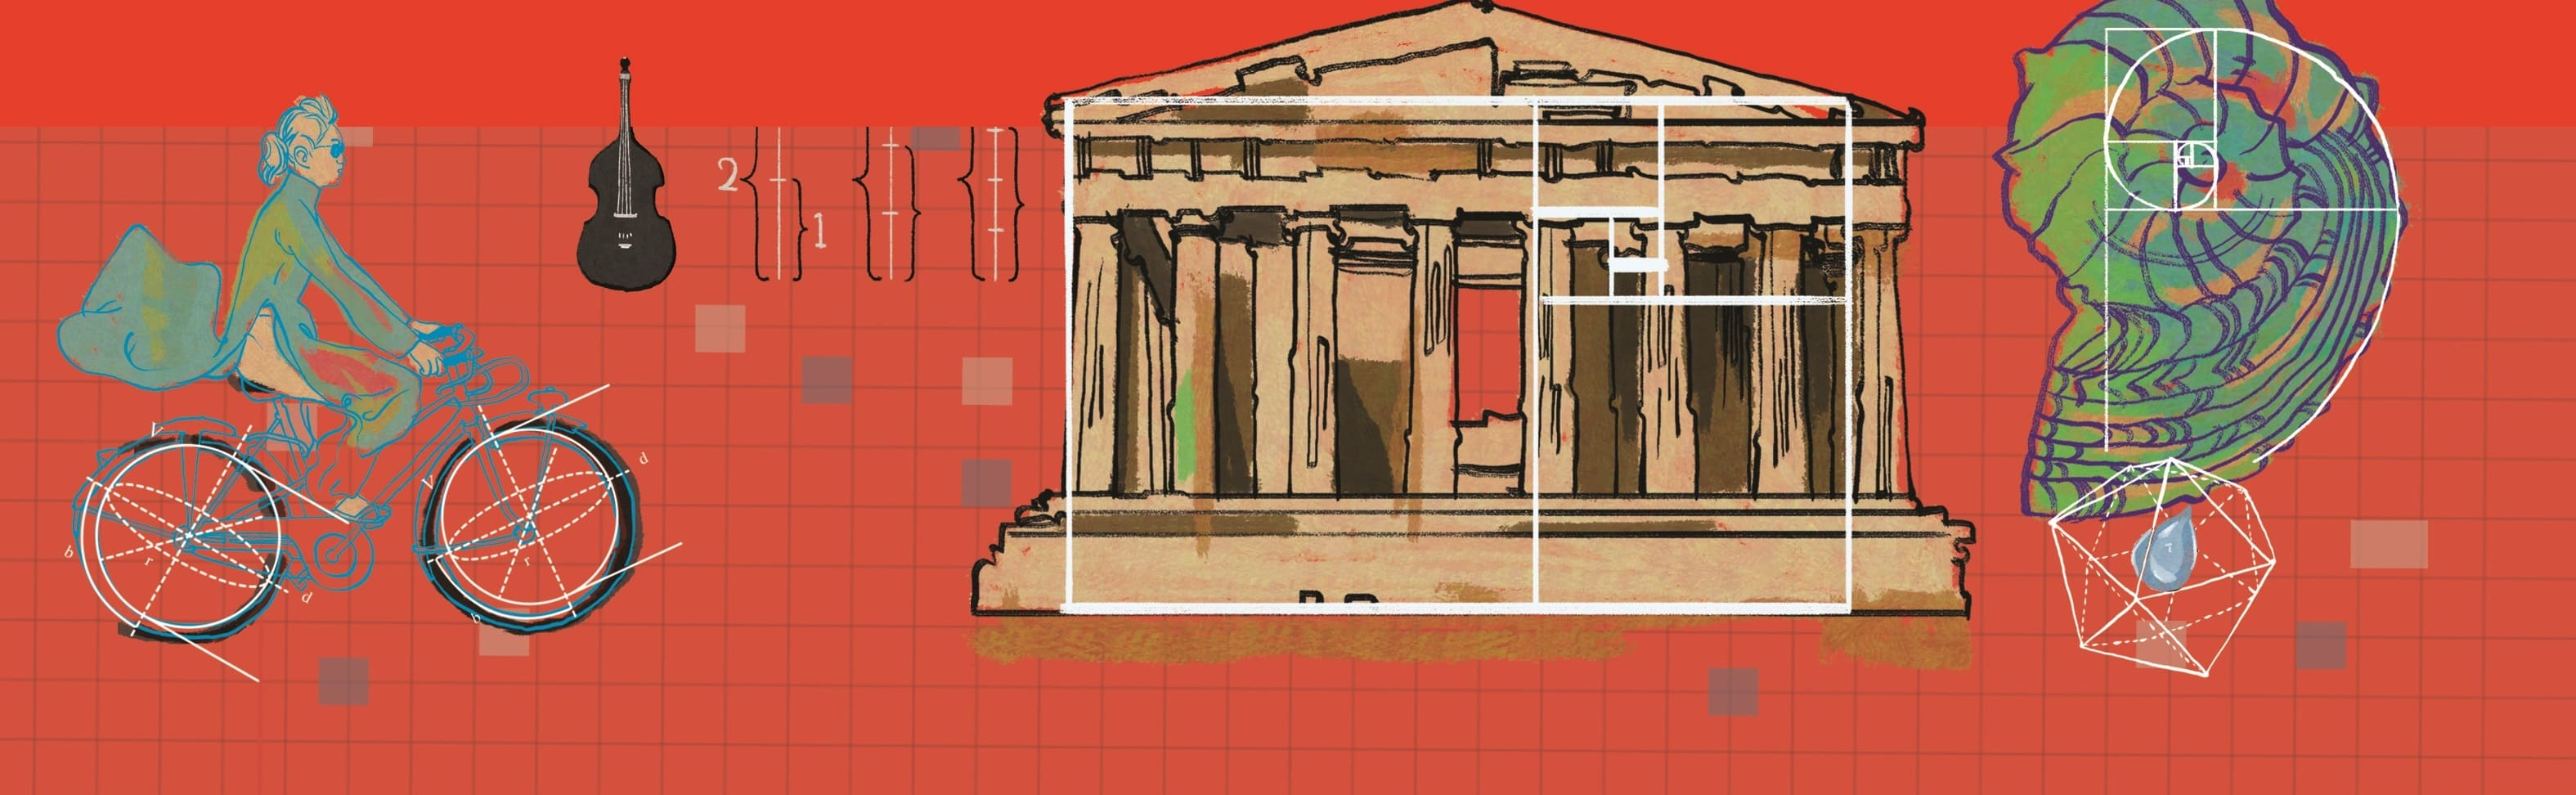
\includegraphics[width=19.3cm]{../bannertoanhocdoisong}}}
\AddToShipoutPicture*{\put(135,540){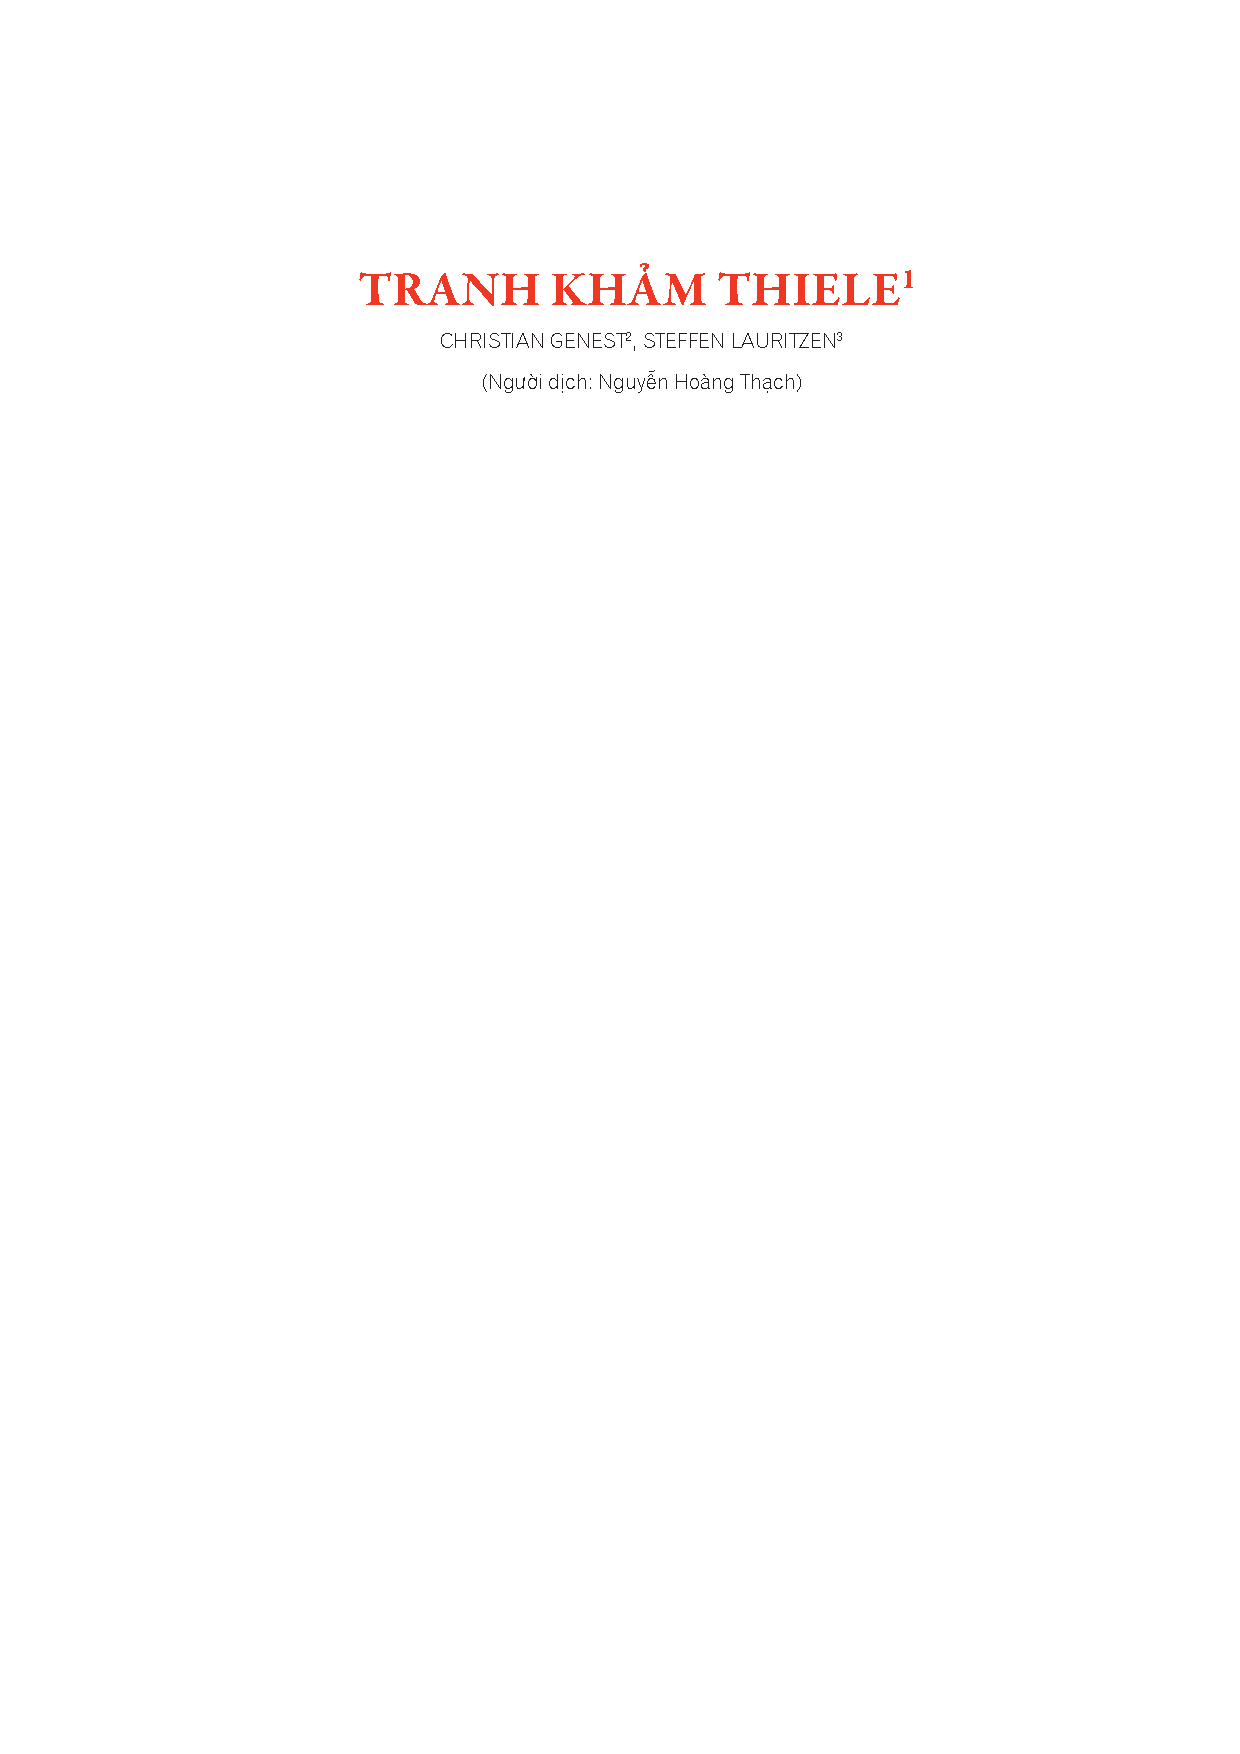
\includegraphics[scale=1]{../tieude2.pdf}}}
\centering
\endgroup

\vspace*{165pt}
\begin{multicols}{2}
	\textit{Nhà thiên văn học, nhà thống kê và doanh nhân bảo hiểm người Đan Mạch Thorvald Thiele đã tìm ra cách sinh tự động các họa tiết khảm rất đẹp nhờ sử dụng khái niệm thặng dư bậc hai trong tập hợp các số nguyên\linebreak Gauss.}
	\vskip 0.1cm
	Tranh khảm gồm nhiều viên hoặc mảnh nhỏ nhiều màu sắc, làm từ những vật liệu khác nhau, được sắp xếp thành một họa tiết trang trí. Được dùng để lát sàn, trang trí tường, trần nhà và các đồ vật, tranh khảm rất được ưa chuộng ở thời Cổ Đại, và vẫn còn được sử dụng trong suốt thời Trung Cổ và Phục Hưng.
	\vskip 0.1cm
	Sau khi gần như biến mất, nghệ thuật lát khảm trở nên phổ biến trở lại với trào lưu nghệ thuật \textit{Art nouveau$^4$}  vào cuối thế kỷ $19$, đầu thế kỷ $20$. Những khám phá khoa học thu hút mạnh mẽ sự chú ý của công chúng và nhiều nghệ sỹ (gồm nhà thơ, nhạc sỹ, họa sỹ, v.v.) đã chuyển tải sức quyến rũ này bằng cách đưa thêm một chiều toán học vào tác phẩm của mình. Sự đều đặn duyên dáng của những họa tiết khảm tô điểm cho những ngôi nhà riêng cũng như những tòa nhà công cộng của chúng ta chỉ là một trong rất nhiều biểu hiện của cuộc tìm tòi thẩm mỹ này.
	\vskip 0.1cm
	Thorvald Thiele ($1838$ -- $1910$) đã đóng góp vào\, trào lưu\, này theo\, cách của\, riêng mình.
	\begin{figure}[H]
		\vspace*{-5pt}
		\centering
		\captionsetup{labelformat= empty, justification=centering}
		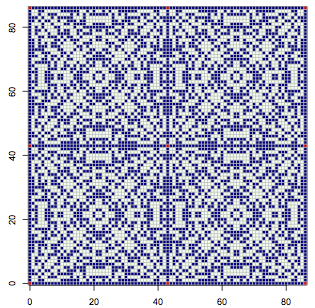
\includegraphics[width= 0.5\linewidth]{mosaique-1.png}
		\caption{\small\textit{\color{toanhocdoisong}Hình $1$. Thặng dư bậc hai modulo $43$.}}
		\vspace*{-10pt}
	\end{figure}
	Ông là người đầu tiên chỉ ra cách sử dụng thặng dư trong tập hợp các số nguyên Gauss để xây dựng một cách dễ dàng những hình khảm tuyệt đẹp. Trong Hình $2$ là hai họa tiết được ông công bố lần đầu tiên tại một hội nghị khoa học lớn của vùng Scandinavia tổ chức tại Copenhagen vào năm $1873$. Còn trong Hình $3$ là họa tiết Thiele ở sàn tiền sảnh Bộ Quốc phòng Đan Mạch, cũng ở Copenhagen.
	\begin{figure}[H]
		\vspace*{-5pt}
		\centering
		\captionsetup{labelformat= empty, justification=centering}
		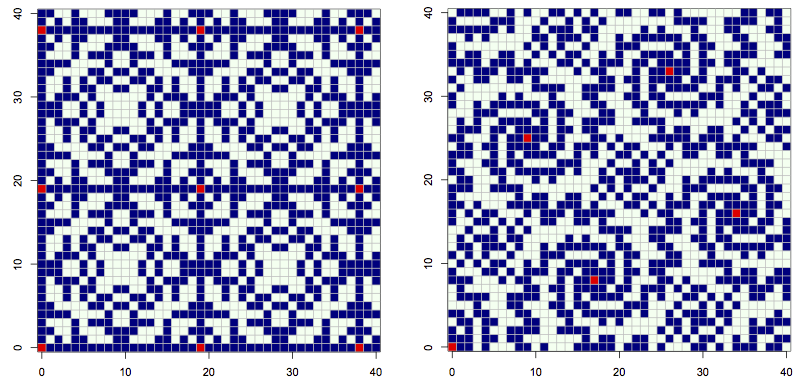
\includegraphics[width= 0.9\linewidth]{mosaique-2.png}
		\caption{\small\textit{\color{toanhocdoisong}Hình $2$. Hai họa tiết được Thiele công bố tại hội nghị khoa học năm $1873$.}}
		\vspace*{-5pt}
	\end{figure}
	Không chỉ tạo ra kết quả tuyệt đẹp, kỹ thuật xây dựng họa tiết khảm của Thiele vừa đơn giản lại vừa khéo léo. Nó dựa trên khái niệm thặng dư bậc hai phức mà chúng ta sẽ cùng nhau tìm hiểu dưới đây. Ở cuối bài, chúng ta sẽ đưa ra ba câu đố chưa có lời giải về họa tiết trong Hình $3$.
	\begin{figure}[H]
		\vspace*{-5pt}
		\centering
		\captionsetup{labelformat= empty, justification=centering}
		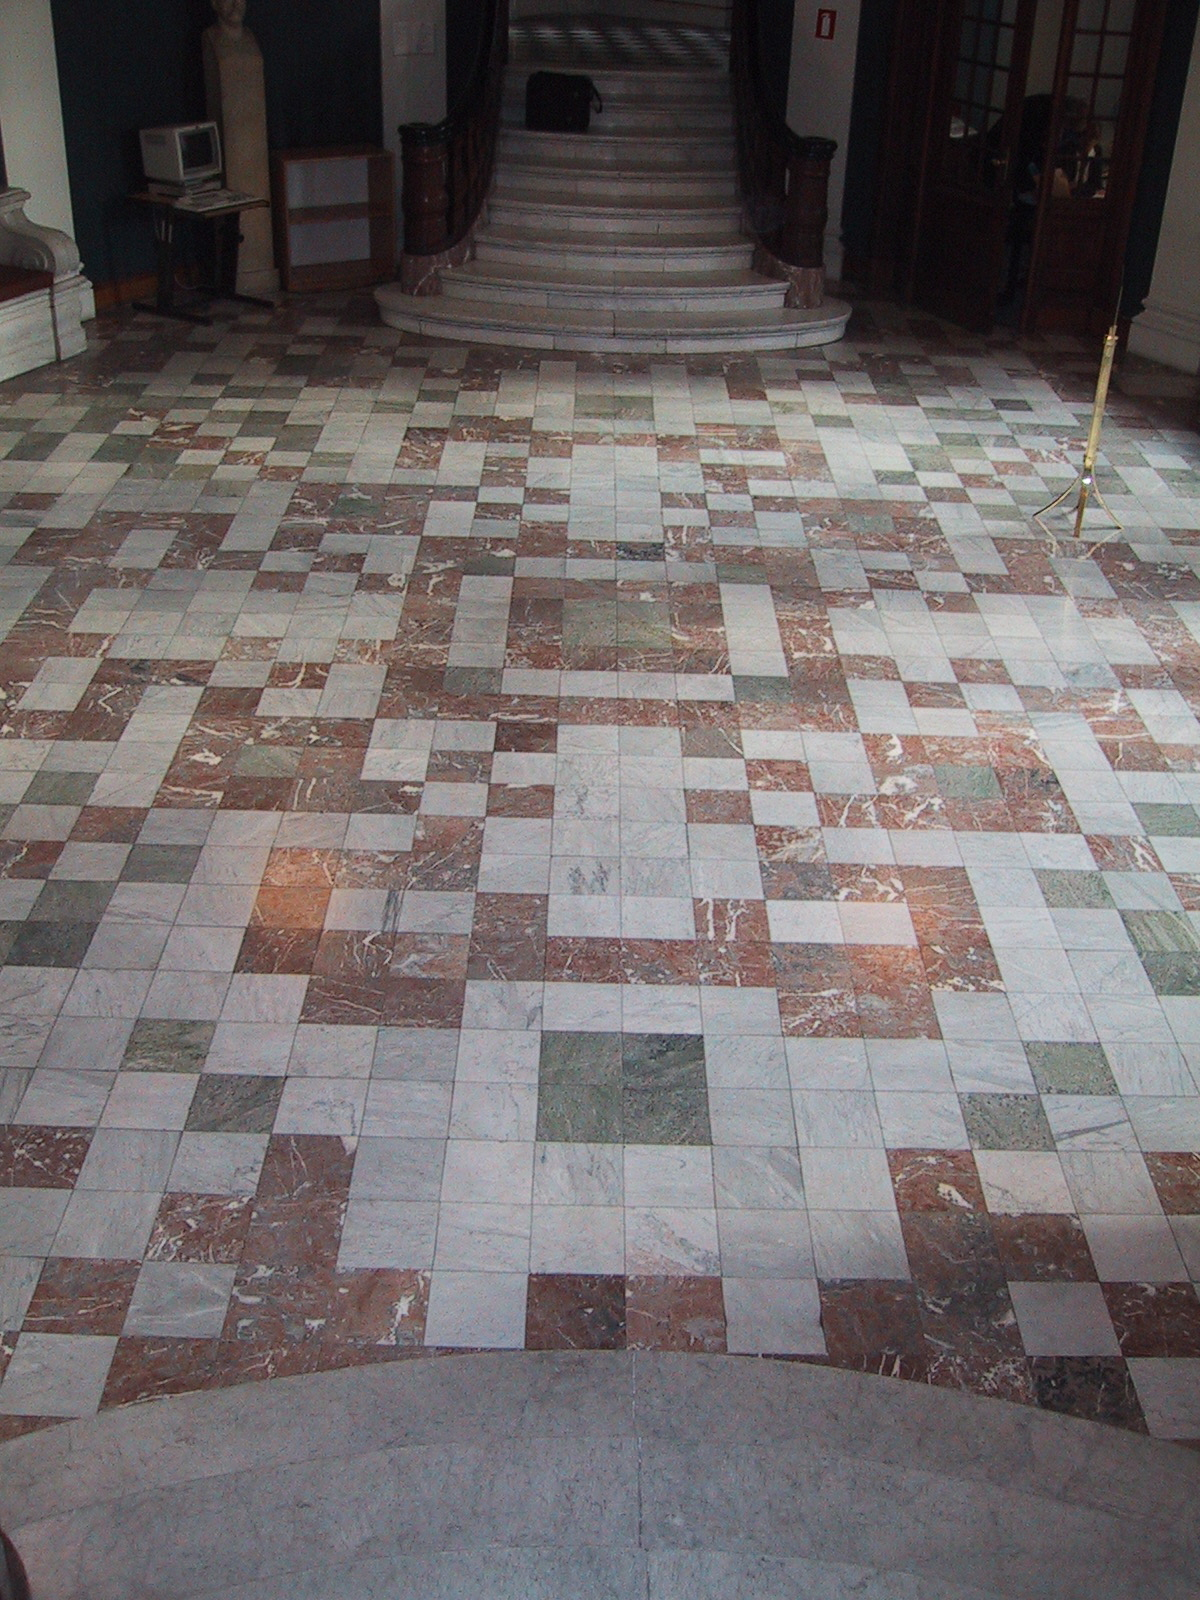
\includegraphics[width= 0.65\linewidth]{mosaique-3}
		\caption{\small\textit{\color{toanhocdoisong}Hình $3$. Họa tiết Thiele trang trí tiền sảnh Bộ Quốc Phòng Đan Mạch, số $9$ phố Holmens Kanal, Copenhagen.}}
		\vspace*{-10pt}
	\end{figure}
	\textbf{\color{toanhocdoisong}Đồng dư và thặng dư bậc hai trong $\pmb{\mathbb Z}$}
	\vskip 0.1cm
	Cho số nguyên $p \ge 1$. Nhắc lại rằng hai số nguyên
	\setlength{\abovedisplayskip}{5pt}
	\setlength{\belowdisplayskip}{5pt}
	\begin{align*}
		a, b \in \mathbb Z = \{ 0, \pm 1, \pm 2, \dots \}
	\end{align*}
	được gọi là đồng dư với nhau modulo $p$ nếu hiệu $a - b$ là bội của $p$, nghĩa là tồn tại $k \in \mathbb Z$ sao cho $a - b = kp$. Khi đó ta viết
	\begin{align*}
		a \equiv b \mod{p}.
	\end{align*}
	Nói riêng, $a$ đồng dư với số dư của nó khi chia cho $p$. Chẳng hạn, ta có thể viết $17 \equiv 1 \mod{4}$ vì $17 - 1 = 16$ chia hết cho $4$, hoặc $28 \equiv 0 \mod{4}$ vì $28 = 4 \times 7$ là bội của $4$.
	\vskip 0.1cm
	Ngoài ra, ta nói rằng số tự nhiên $q \in \mathbb N = \{ 0, 1, 2, \dots \}$ là một {\em thặng dư bậc hai} modulo $p$ nếu tồn tại số nguyên $x$ sao cho
	\begin{align*}
		q \equiv x^2 \mod{p}.
	\end{align*}
	Trong trường hợp ngược lại, ta nói $q$ không phải là thặng dư bậc hai modulo $p$.
	\vskip 0.1cm
	\textbf{\color{toanhocdoisong}Hai ví dụ đơn giản}
	\vskip 0.1cm
	\textbf{\color{toanhocdoisong}Ví dụ} $1.$ Mọi số tự nhiên $q$ đều là thặng dư bậc hai modulo $2$. Thật vậy:
	\vskip 0.1cm
	$\bullet$	Nếu $q \equiv 0 \mod{2}$, tức $q$ chẵn, thì $q \equiv 0^2 \mod{2}$;
	\vskip 0.1cm
	$\bullet$	Nếu $q \equiv 1 \mod{2}$, tức $q$ lẻ, thì $q \equiv 1^2 \mod{2}$.
	Một cách tổng quát, với mọi $p$, mọi số tự nhiên $q$ đồng dư với $0$ hoặc $1$ đều là thặng dư bậc hai modulo $p$.
	\vskip 0.1cm
	\textbf{\color{toanhocdoisong}Ví dụ} $2.$
	\vskip 0.1cm
	$\bullet$	Nếu $q \equiv 0 \mod{4}$, thì $q \equiv 0^2 \mod{4}$;
	\vskip 0.1cm
	$\bullet$	Nếu $q \equiv 1 \mod{4}$, thì $q \equiv 1^2 \mod{4}$.
	\vskip 0.1cm
	Trong khi đó, nếu $q \equiv 2 \mod{4}$ hoặc $q \equiv 3 \mod{4}$, không tồn tại số nguyên $x$ nào sao cho $q \equiv x^2 \mod{4}$. Điều này có thể được chứng minh bằng cách xét hai trường hợp $x$ chẵn và $x$ lẻ:
	\vskip 0.1cm
	$\bullet$	Nếu $x = 2n$ thì $x^2 = 4 n^2 \equiv 0 \mod{4}$;
	\vskip 0.2cm
	$\bullet$	Nếu $x = 2n + 1$ thì $x^2 = 4 n^2 + 4n + 1 \equiv 1 \mod{4}$.
	\vskip 0.2cm
	\textbf{\color{toanhocdoisong}Vỉa hè Thiele}
	\vskip 0.2cm
	Kết quả trên được minh họa trong Hình $4$ bằng ``vỉa hè Thiele". Một cách tổng quát, vỉa hè Thiele modulo $p$ gồm các mảnh hình vuông đơn vị đặt chính giữa các điểm $(0, 0)$, $(1, 0)$, $(2, 0)$, v.v. Màu của mảnh hình vuông tại điểm $(q, 0)$ được xác định như sau:
	\vskip 0.1cm
	$\bullet$	đỏ nếu $q \equiv 0 \mod{p}$;
	\vskip 0.1cm
	$\bullet$	xanh nếu $q$ là thặng dư bậc hai modulo $p$ (nhưng $q \not\equiv 0 \mod{p}$);
	\vskip 0.1cm
	$\bullet$	trắng nếu $q$ không phải thặng dư bậc hai modulo $p$.
	\begin{figure}[H]
		\vspace*{-5pt}
		\centering
		\captionsetup{labelformat= empty, justification=centering}
		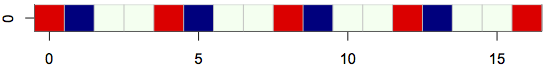
\includegraphics[width= 1\linewidth]{mosaique-4.png}
		\caption{\small\textit{\color{toanhocdoisong}Hình $4$. Vỉa hè Thiele modulo $4$.}}
		\vspace*{-10pt}
	\end{figure}
	Khi $p = 4$, mọi số tự nhiên $q$ đồng dư với $0$, $1$, $2$ hoặc $3$ modulo $4$. Họa tiết ``đỏ, xanh, trắng, trắng" ứng với các mảnh $(0, 0)$, $(1, 0)$, $(2, 0)$, $(3, 0)$ lặp lại vô hạn. Với mọi giá trị $p \ge 1$ khác, vỉa hè Thiele modulo $p$ có thể được xây dựng dễ dàng một khi ta đã biết màu của các mảnh $(0, 0), \dots, (p - 1, 0)$: họa tiết lặp lại với chu kỳ $p$.
	\vskip 0.2cm
	Các họa tiết khảm Thiele dựa trên một nguyên lý tương tự. Với mỗi cặp số nguyên $p = (p_1, p_2)$, màu của mảnh $(q_1, q_2)$ sẽ phụ thuộc vào việc $(q_1, q_2)$ có phải là thặng dư bậc hai modulo $p$ hay không. Để điều này có nghĩa, trước tiên chúng ta cần tìm hiểu khái niệm đồng dư giữa hai cặp số nguyên.
	\begin{tBox}
		\textbf{\textit{\color{toanhocdoisong}Thorvald Nicolai Thiele $\pmb{(1838 \!-\! 1910)}$}}
		\vskip 0.2cm
		\begin{wrapfigure}{l}{0.4\textwidth}
			\vspace*{-14pt}
			\centering
			\captionsetup{labelformat= empty, justification=centering}
			\hspace*{3pt}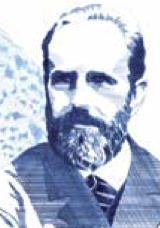
\includegraphics[width= 1.1\linewidth]{Thiele.png}
			\vspace*{-20pt}
		\end{wrapfigure}
		Thorvald Thiele sinh ngày $24$ tháng $12$ năm $1838$ ở Copenhagen và mất ngày $26$ tháng $9$ năm $1910$ ở cùng thành phố, thọ $71$ tuổi. Tên ông được đặt theo cha đỡ đầu của ông, nhà điêu khắc Bertel Thorvaldsen. Sau quá trình học tập xuất sắc, ông trở thành giáo sư thiên văn học tại Đại học Copenhagen từ năm $1875$ đến năm $1907$, đồng thời là giám đốc đài thiên văn của trường. Được coi là một người mở đường của thống kê toán học, ông là người đầu tiên đề xuất một lý thuyết chuyển động Brown, đồng thời là tác giả của các khái niệm cumulant và hàm hợp lý. Thiele cũng góp phần sáng lập Hafnia, công ty bảo hiểm nhân thọ tư nhân đầu tiên của của Đan Mạch, vào năm $1872$. Ông là giám đốc khoa học của công ty tới năm $1901$, rồi chủ tịch Hội đồng Quản trị từ năm $1903$ tới năm $1910$. Tên ông được đặt cho hai tiểu hành tinh; một trong  hai tiểu hành tinh đó được phát hiện bởi con trai ông, Holger Thiele, cũng là một nhà thiên văn học nổi tiếng.
	\end{tBox}
	\textbf{\color{toanhocdoisong}Mở rộng cho tập hợp các số nguyên Gauss}
	\vskip 0.1cm
	Trong công trình \textit{Disquisitiones arithmeticae\footnote[5]{\color{toanhocdoisong}Công ty phá sản năm $1993$.}}  xuất bản năm $1801$, nhà toán học, vật lý học và thiên văn học người Đức Carl Friedrich Gauss ($1777$ -- $1855$) quan tâm đến số học đồng dư trên những tập hợp khác $\mathbb Z$, trong đó có tập hợp các cặp số nguyên, tức là các vector $(a_1, a_2) \in \mathbb Z^2 = \mathbb Z \times \mathbb Z$.
	\vskip 0.1cm
	Gauss định nghĩa tổng và tích của hai phần tử bất kỳ $a = (a_1, a_2)$, $b = (b_1, b_2)$ trong $\mathbb Z^2$ như sau:
	\begin{align*}
		&(a_1, a_2) + (b_1, b_2) \\
		= \,&(a_1 + b_1, a_2 + b_2), \\
		&(a_1, a_2) \times (b_1, b_2) \\
		= \,&(a_1  b_1 - a_2  b_2, a_1  b_2 + a_2  b_1).
	\end{align*}
	Phép cộng là phép cộng vector thông thường. Phép nhân, có vẻ bí ẩn hơn, liên hệ mật thiết với khái niệm số phức (xem phần đóng khung bên dưới).
	\vskip 0.1cm
	Tập hợp $\mathbb Z^2$ được trang bị hai phép toán trên được gọi là tập hợp các {\em số nguyên Gauss}. Tập hợp các số nguyên Gauss có đủ các tính chất cần thiết để ta có thể định nghĩa trên đó các khái niệm đồng dư và thặng dư bậc hai tương tự những khái niệm đã có trên $\mathbb Z$.
	\vskip 0.1cm
	Cho hai số tự nhiên $p_1$ và $p_2$ không đồng thời bằng $0$. Ta nói rằng hai phần tử $a, b \in \mathbb Z$ đồng dư với nhau modulo $p = (p_1, p_2)$ nếu tồn tại $k = (k_1, k_2) \in \mathbb Z^2$ sao cho $a - b = k \times p$. Nói cách khác, $a \equiv b \mod{p}$ nếu và chỉ nếu
	\begin{align*}
		&(a_1, a_2) - (b_1, b_2) \\
		= \,&(k_1 p_1 - k_2 p_2, k_1 p_2 + k_2 p_1).
	\end{align*}
	Ta nói rằng $q = (q_1, q_2)$ là một {\em thặng dư bậc hai phức} modulo $p = (p_1, p_2)$ nếu tồn tại $x = (x_1, x_2) \in \mathbb Z^2$ sao cho $q \equiv x^2 \mod{p}$. Nói cách khác, ta cần tìm các số nguyên $x_1$ và $x_2$ sao cho
	\begin{align*}
		(q_1, q_2) \equiv (x_1^2 - x_2^2, 2 x_1 x_2) \mod{p}.
	\end{align*}
	\vskip 0.1cm
	\begin{tBox}
		\textbf{\textit{\color{toanhocdoisong}Mối liên hệ với số phức}}
		\vskip 0.1cm
		\begin{wrapfigure}{r}{0.4\linewidth}
			\vspace*{-15pt}
			\centering
			\captionsetup{labelformat= empty, justification=centering}
			\hspace*{-12pt}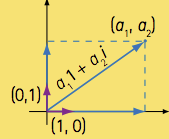
\includegraphics[width= 1.15\linewidth]{mosaique-6.png}
			\vspace*{-15pt}
		\end{wrapfigure}
		Các phép toán được Gauss định nghĩa trong $\mathbb Z^2$ có liên hệ mật thiết với khái niệm số phức. Một số phức là một số có dạng $a_1 + a_2 i$, ở đó $i = \sqrt{-1}$. Số phức có thể được biểu diễn trong mặt phẳng bằng cách đặt $1 = (1, 0)$ và $i = (0, 1)$, sao cho $(a_1, a_2) = a_1 1 + a_2 i$, mà ta có thể viết gọn là $a_1 + a_2 i$ mà không sợ nhầm lẫn. Thực hiện phép cộng và phép nhân thông thường với các biểu thức đại số $a_1 + a_2 i$ và $b_1 + b_2 i$, ta được:
		\begin{align*}
			&(a_1 + a_2 i) + (b_1 + b_2i) \\
			= \,&(a_1 + b_1) + (a_2 + b_2) i, \\
			&(a_1 + a_2i) \times (b_1 + b_2i) \\
			= \,&a_1 b_1 + (a_1 b_2 + a_2 b_1) i + a_2 b_2 i^2 \\
			= \,&( a_1  b_1 - a_2  b_2) + (a_1 b_2 + a_2 b_1) i ,
		\end{align*}
		ở đó ta đã thay $i^2 = -1$.
		\vskip 0.1cm
		Để ý rằng phép nhân với $i$ tương đương với phép quay một góc $\pi / 2$ ngược chiều kim đồng hồ. Thật vậy:
		\begin{align*}
			(a_1 + a_2 i) \times i = a_1 i + a_2 i^2 = -a_2 + a_1 i.
		\end{align*}
		\begin{wrapfigure}{r}{0.4\linewidth}
			\vspace*{-15pt}
			\centering
			\captionsetup{labelformat= empty, justification=centering}
			\hspace*{-12pt}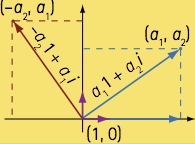
\includegraphics[width= 1.1\linewidth]{mosaique-7.png}
			\vspace*{-15pt}
		\end{wrapfigure}
		Khi $a_2 = 0$, số là {\em số thực}, còn khi $a_1 = 0$, số là {\em số ảo}.
		Các phép toán được định nghĩa trong tập hợp các số phức chính là các phép toán trong tập hợp các số nguyên Gauss. Tập hợp $\mathbb Z^2$ cùng với hai phép toán này thường được ký hiệu là $\mathbb Z[i]$.
	\end{tBox}
	\vskip 0.1cm
	\textbf{\color{toanhocdoisong}Hình khảm Thiele}
	\vskip 0.1cm
	Cũng như vỉa hè Thiele, một hình khảm Thiele modulo $p = (p_1, p_2)$ gồm nhiều mảnh hình vuông đơn vị phủ kín mặt phẳng. Màu của mảnh tại điểm $q = (q_1, q_2)$ được xác định như sau:
	\vskip 0.1cm
	$\bullet$	đỏ nếu $q \equiv 0 \mod{p}$;
	\vskip 0.1cm
	$\bullet$	xanh nếu $q$ là thặng dư bậc hai phức modulo $p$ (nhưng $q \not\equiv 0 \mod{p}$);
	\vskip 0.1cm
	$\bullet$	trắng nếu $q$ không phải thặng dư bậc hai phức modulo $p$.
	\vskip 0.1cm
	Ví dụ, giả sử $p = (2, 0)$. Ta có:
	\begin{align*}
		&(a_1, a_2) \equiv (b_1, b_2) \mod{p} \\
		\iff& a_1 - b_1 = 2 k_1 \mbox{ và } a_2 - b_2 = 2 k_2,
	\end{align*}
	tức là $a_1 \equiv b_1 \mod{2}$ và $a_2 \equiv b_2 \mod{2}$. Suy ra với mọi $(a_1, a_2) \in \mathbb Z^2$, $(a_1, a_2) \equiv (0, 0), (0, 1), (1, 0)$ hoặc $(1, 1) \mod{p = (2, 0)}$.
	\vskip 0.1cm
	Từ nhận xét trên, để xây dựng hình khảm Thiele tương ứng, ta chỉ cần xét xem $(0, 0), (0, 1), (1, 0)$ và $(1, 1)$ có phải thặng dư bậc hai phức modulo $p = (2, 0)$ hay không.
	\vskip 0.1cm
	Như vậy, với $a_1, a_2 \in \{0, 1\}$, ta cần kiểm tra xem có tồn tại hay không $x_1, x_2 \in \mathbb Z$ sao cho
	\begin{align*}
		a_1 \equiv x_1^2 - x_2^2 \mod{2}, a_2 \equiv 2 x_1 x_2 \mod{2}.
	\end{align*}
	Nếu $a_2 = 0$, chỉ cần chọn $x_1 = a_1$ và $x_2 = 0$. Nhưng nếu $a_2 = 1$ thì không thể tìm được $x_1, x_2 \in \mathbb Z$ thỏa mãn vì $2 x_1 x_2$ luôn chẵn.
	\vskip 0.1cm
	Kết quả này được mình họa trong Hình $5$. Các mảnh $(0, 0)$, $(1, 0)$, $(0, 1)$ và $(1, 1)$ tạo thành họa tiết cơ bản (bên trái) mà chúng ta có thể lặp lại một số lần tùy ý (bên phải). Hiệu ứng ảo giác của hình vẽ được tạo bởi sự tuần hoàn kép (cả chiều ngang lẫn chiều dọc) của họa tiết cùng với các màu sắc tương phản mạnh.
	\begin{figure}[H]
		\vspace*{-5pt}
		\centering
		\captionsetup{labelformat= empty, justification=centering}
		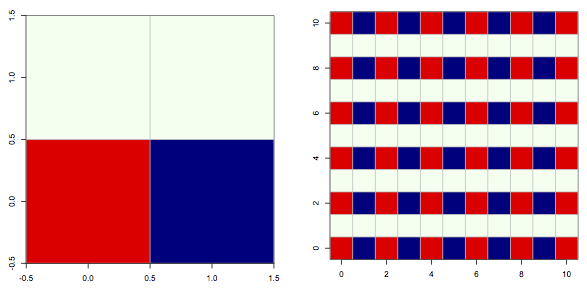
\includegraphics[width= 1\linewidth]{mosaique-8.png}
		\caption{\small\textit{\color{toanhocdoisong}Hình $5$. Hình khảm Thiele modulo $p = (2, 0)$.}}
		\vspace*{-10pt}
	\end{figure}
	Hai thí dụ khác, do chính Thiele đưa ra, được trình bày trong Hình $2$ (hình này được vẽ bằng một phần mềm miễn phí, với hướng dẫn tải và sử dụng ở cuối bài). Hình khảm bên trái tương ứng với $p = (19, 0)$; có thể dễ dàng nhận thấy nó tuần hoàn theo chiều dọc và chiều ngang. Hình khảm bên phải tương ứng với $p = (17, 8)$; chúng ta cũng nhận có sự đều đặn, nhưng việc xác định chính xác nó thì không hiển nhiên như trường hợp trước.
	\vskip 0.1cm
	\textbf{\color{toanhocdoisong}Ý nghĩa hình học}
	\vskip 0.1cm
	Để hiểu rõ hơn quy luật của hình khảm Thiele, chúng ta hãy coi các phần tử của $\mathbb Z^2$ như các vector tọa độ nguyên. Để ý rằng theo định nghĩa, hai vector $a = (a_1, a_2)$ và $b = (b_1, b_2)$ đồng dư với nhau modulo $p = (p_1, p_2)$ nếu và chỉ nếu
	\begin{align*}
		&(a_1, a_2) - (b_1, b_2) \\
		= \,&(k_1 p_1 - k_2 p_2, k_1 p_2 + k_2 p_1) \\
		= \,&k_1 (p_1, p_2) + k_2 (-p_2, p_1) ,
	\end{align*}
	nghĩa là nếu hiệu của chúng có thể viết thành tổng của một bội của $p$ và một bội của vector $p' = (-p_2, p_1)$ vuông góc với $p$.
	\vskip 0.1cm
	Trong ngôn ngữ hình học, điều này có nghĩa là hai vector $a$ và $b$ đồng dư với nhau modulo $p$ nếu có thể đi từ $a$ tới $b$ (hoặc ngược lại) bằng một số hữu hạn các tịnh tiến theo $p$, $-p$, $p'$ và $-p'$. Đặc biệt, tất cả các vector [trong $\mathbb Z^2$] đều đồng dư với một vector nằm trong hình vuông có bốn đỉnh $(0, 0)$, $p$, $p'$ và $p + p'$. Tính chất này là tương đương trong $\mathbb Z^2$ của phép chia có dư trong $\mathbb Z$.
	\vskip 0.1cm
	Quay trở lại với hình bên phải của Hình $2$, chúng ta có thể kiểm tra rằng họa tiết cơ bản quả đúng là phần được giới hạn bởi bốn điểm đỏ $(9, 25)$, $(17, 8)$, $(26, 33)$ và $(34, 16)$.
	\vskip 0.1cm
	\PIbox{\textbf{\color{toanhocdoisong}\textit{Có bao nhiêu mảnh được tô màu?}}
		\vskip 0.1cm
		Kinh nghiệm cho thấy những hình khảm Thiele đẹp nhất khi $p = (p_1, p_2)$ là một {\em số nguyên tố Gauss}, nghĩa là nếu với mọi $a, b \in \mathbb Z^2$:
		\begin{align*}
			&a \times b \equiv (0, 0) \mod{p} \\
			\implies &a \equiv (0, 0) \mbox{ hoặc } b \equiv (0, 0) \mod{p}.
	\end{align*}}
	\PIbox{
		Có thể chứng minh được rằng $p$ là số nguyên tố Gauss nếu và chỉ nếu một trong ba điều kiện sau được thỏa mãn (chúng ta thừa nhận kết quả này):
		\vskip 0.1cm
		$\bullet$	Nếu $p_1 \ge 1$ và $p_2 \ge 1$: $p_1^2 + p_2^2$ là số nguyên tố theo nghĩa thông thường;
		\vskip 0.1cm
		$\bullet$	Nếu $p_1 = 0$ và $p_2 \ge 1$: $|p_2|$ nguyên tố và $|p_2| \equiv 3 \mod{4}$;
		\vskip 0.1cm
		$\bullet$	Nếu $p_1 \ge 1$ và $p_2 = 0$: $|p_1|$ nguyên tố và $|p_1| \equiv 3 \mod{4}$.
		\vskip 0.1cm
		Như vậy, $(19, 0)$, $(71, 0)$ và $(17, 8)$ là các số nguyên tố Gauss, nhưng $(5, 0)$ thì không phải, và ta có $(5, 0) = (1, 2) \times (1, -2)$.
		\vskip 0.1cm
		Ta biết rằng nếu $p$ là một số nguyên tố, một nửa các số từ $1$ đến $p - 1$ là thặng dư bậc hai modulo $p$. Nói cách khác, có $(p - 1) / 2$ mảnh màu xanh trong họa tiết cơ bản của vỉa hè Thiele modulo $p$. Tương tự, bằng cách sử dụng các khái niệm trong lý thuyết trường, có thể chứng minh rằng nếu $p = (p_1, p_2)$ là số nguyên tố Gauss với $p_1 \ge 1$ và $p_2 \ge 1$, thì có $p_1^2 + p_2^2 - 1$ mảnh màu xanh trong họa tiết cơ bản của hình khảm Thiele modulo $p$.}
	\vskip 0.2cm
	\textbf{\color{toanhocdoisong}Trở lại bức hình tiền sảnh}
	\vskip 0.1cm
	Sàn sảnh trong Hình $3$ được lát theo hình khảm Thiele modulo $(71, 0)$. Họa tiết cơ bản của nó được cho trong Hình $6$. Ngày nay thuộc Bộ Quốc phòng Đan Mạch, tòa nhà có sàn lát này từng là trụ sở của công ty bảo hiểm Hafnia. Ở cương vị chủ tịch Hội đồng Quản trị của công ty, Thiele đã cho phép khởi công xây tòa nhà vào tháng $5$ năm $1910$, chỉ vài tháng trước khi ông qua đời ở tuổi $71$. Người ta cho rằng họa tiết lát sảnh được chọn sau khi Thiele mất, để tưởng nhớ ông.
	\vskip 0.1cm
	Chúng ta có thể rút ra ba quan sát về hình lát sàn này như sau:
	\vskip 0.1cm
	$\bullet$ Có một số lỗi trong việc thể hiện họa tiết. Thực vậy, mặc dù $(27, 35)$ là thặng dư bậc hai modulo $p = (71, 0)$, viên gạch lát tương ứng lại có màu trắng. Đây có thể là một lỗi tính toán, vì nó xuất hiện đến bảy lần trên toàn bộ tác phẩm.
	\begin{figure}[H]
		\vspace*{-5pt}
		\centering
		\captionsetup{labelformat= empty, justification=centering}
		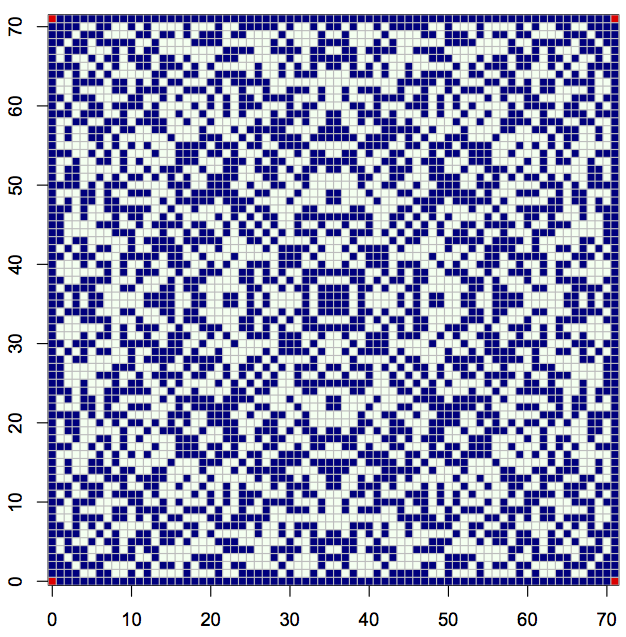
\includegraphics[width= 0.85\linewidth]{mosaique-9.png}
		\caption{\small\textit{\color{toanhocdoisong}Hình $6$. Hình khảm Thiele modulo $(71, 0)$, được dùng làm mẫu lát sàn tiền sảnh Bộ Quốc phòng Đan Mạch.}}
		\vspace*{-10pt}
	\end{figure}
	$\bullet$ Khi so sánh Hình $3$ và Hình $6$, chúng ta thấy mảnh $(25, 45)$ đúng ra phải màu trắng, nhưng trên sàn gạch thực tế lại màu đỏ. Lỗi này không lặp lại ở những chỗ khác. Không rõ đây là do sự lơ đãng của người thợ lát, hay do truyền thống nghề nghiệp không muốn sự hoàn hảo?
	\begin{figure}[H]
		\vspace*{-5pt}
		\centering
		\captionsetup{labelformat= empty, justification=centering}
		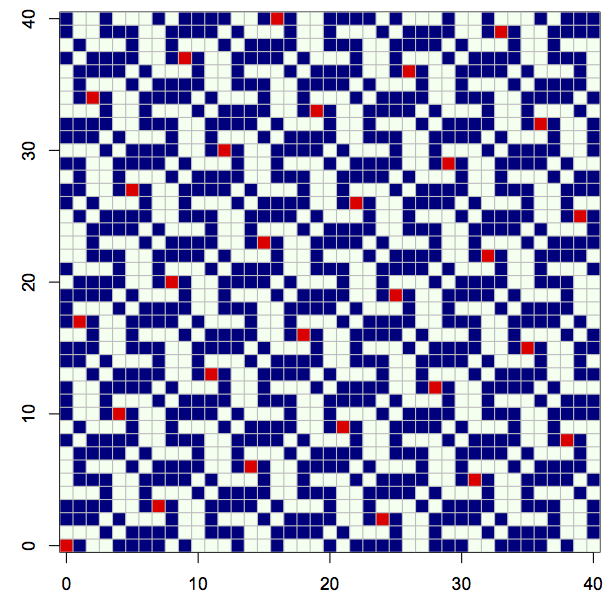
\includegraphics[width= 0.85\linewidth]{mosaique-10.png}
		\caption{\small\textit{\color{toanhocdoisong}Hình $7$. Thặng dư bậc hai modulo $(7, 3)$. Hình khảm này được tạo với một số không nguyên tố: $(7, 3) = (1, -1) \times (2, 5)$.}}
		\vspace*{-10pt}
	\end{figure}
	$\bullet$ Vì sao một số viên gạch tương ứng với thặng dư bậc hai có màu đỏ, trong khi những viên khác lại xanh lá cây? Liệu có phải chỉ đơn giản vì lý do thẩm mỹ? Tính cân đối của họa tiết gợi ý rằng hai màu này thể hiện một tính chất khác của các thặng dư bậc hai. Nhưng đó là tính chất gì?
	\vskip 0.1cm
	Có thể lục lại các tài liệu lưu trữ của công ty Hafnia để tìm câu trả lời cho hai câu hỏi đầu tiên. Câu hỏi thứ ba thì có bản chất thuần túy toán học và việc giải đáp nó có thể cần đến các tính chất của các số nguyên Gauss, của thặng dư bậc hai (hay bậc bốn?) phức và các chủ đề hấp dẫn khác của lý thuyết số. Câu trả lời vẫn là bí ẩn, và việc tìm ra nó được dành cho các bạn!
	\vskip 0.2cm
	\PIbox{
	\textbf{\color{toanhocdoisong}\textit{Vẽ tranh khảm Thiele bằng R}}
	\vskip 0.1cm
	Chúng ta có thể dễ dàng tạo ra một hình khảm Thiele nhờ một chương trình được viết bởi S{\o}ren Buhl, giáo sư toán và thống kê, Đại học Aalborg (Đan Mạch). Chương trình của ông được viết bằng ngôn ngữ R, có thể được tải miễn phí cho Windows, MacOS hoặc Linux tại:
	\url{http://www.r-project.org/}
	\vskip 0.1cm
	Chương trình vẽ có thể được tải ở đây:
	\url{http://www.math.mcgill.ca/cgenest/Thiele.R}
	\vskip 0.1cm
	Sau khi sao chép đoạn mã của chương trình vào cửa sổ lệnh của R, ta có thể vẽ một hình khảm Thiele modulo $p$ với kích thước $(n + 1) \times (n + 1)$ bằng lệnh $tuile(p, n)$. Thí dụ, Hình $2$ là kết quả của các lệnh $tuile(19,40)$ và $tuile(17 + 8i, 40)$. Hình $5$ nhận được bằng cách nhập lệnh $tuile(71, 71)$.}
	\vskip 0.1cm
	\textbf{\color{toanhocdoisong}Tài liệu tham khảo}
	\vskip 0.1cm
	[$1$] Décaillot, A.--M. ($2002$). Géométrie des tissus, mosaïques, échiquiers: Mathématiques curieuses et utiles. \textit{Revue d'histoire des mathématiques}, vol. $8$, pp. $145-206$.
	\vskip 0.1cm
	[$2$] Lauritzen, S., \textit{Thiele: Pioneer in Statistics}, Oxford University Press, $2002$.
\end{multicols}